\RequirePackage[T1]{fontenc}
\documentclass[conference]{IEEEtran}
\usepackage{cite,amsmath,amssymb,graphicx,booktabs,url,balance}
\usepackage[hidelinks]{hyperref}
\hyphenation{classi-fi-ca-tion cali-bra-tion}
\begin{document}
\title{Smart Waste Segregation Assistant:\\Handcrafted Features and Calibrated Classical Classification}
\author{\IEEEauthorblockN{Om Yadav, Aditya Bharadwaj, Shourya Bafna,\\Daksh Batra, Prajjwal Tripathi, Saksham Mighlani}
\IEEEauthorblockA{CSAI Project 12 --- Phase 1: Machine Learning\\26 October 2026}}
\maketitle
\pagestyle{plain}
\thispagestyle{plain}
\begin{abstract}
This project implements an educational photo classifier for six TrashNet material categories using classical machine learning. An audit excludes six images with conflicting duplicate labels and partitions 2,521 usable images into 1,764 training, 380 validation and 377 test images while keeping detected duplicate groups together. We compare support vector machines and random forests using handcrafted color, gradient and texture descriptors. The selected RBF SVM uses 1,608 color and spatial texture features from a 2,760-dimensional extractor, with square-root and per-image $L_2$ normalization. It achieves mean training cross-validation macro F1 of $0.8803\pm0.0215$ across five frozen folds. A group-aware sigmoid-calibrated ensemble and a validation-selected abstention threshold of 0.52 achieve test macro F1 of 0.8999 and accuracy of 90.19\%. Accepting 371 of 377 test images yields 91.37\% accepted accuracy. The local demonstration presents six probabilities and an uncertainty response. These results describe this controlled dataset split, not general waste-disposal reliability. We document calibration error, incomplete same-item detection, background sensitivity and historical source-provenance limits.
\end{abstract}
\begin{IEEEkeywords}
Waste classification, handcrafted features, SVM, random forest, calibration, selective classification.
\end{IEEEkeywords}

\section{Problem and Scope}
The objective is to suggest a visual material class from a photograph: cardboard, glass, metal, paper, plastic or trash. These labels are not universal recycling instructions. Local rules, contamination and mixed materials determine actual disposal decisions. Phase~1 covers handcrafted descriptors, classical models, fair comparison, confidence calibration and an educational upload prototype. Transfer learning is planned for Phase~2 and is not part of the reported implementation.

The central question is whether engineered color and texture features can support useful classification while retaining a reproducible evaluation protocol. We measure macro F1 to give each class equal weight, inspect class recall, and separate model selection from the final test evaluation. All numerical results in this report come from saved project records; preparing this report did not retrain a model or rerun final test inference.

\section{Related Work and Method Rationale}
Thung and Yang's TrashNet project provides a six-category benchmark photographed largely against a white background~\cite{yang2016trashnet}. Its controlled capture conditions make it a useful starting point, but they do not represent the full variety of everyday scenes. We therefore treat external generalization as an open evaluation question.

Histogram of Oriented Gradients (HOG) aggregates local edge orientation and uses block normalization~\cite{dalal2005hog}. Local Binary Patterns (LBP) encode neighborhood intensity comparisons and provide compact texture histograms~\cite{ojala2002lbp}. Color histograms complement these descriptors by representing material appearance, although lighting and background can influence them. Our experiments compare feature families rather than assuming that concatenating every descriptor improves performance.

Support vector machines (SVMs) seek margin-based decision boundaries and can use nonlinear kernels~\cite{cortes1995svm}. Random forests aggregate randomized decision trees~\cite{breiman2001randomforest}. The two families provide different inductive biases and let us test both scaled histogram representations and tree-based feature interactions.

Platt scaling maps classifier scores through a sigmoid~\cite{platt1999probabilistic}. Niculescu-Mizil and Caruana distinguish accurate classification from accurate probabilities and study calibration methods~\cite{niculescu2005predicting}. Selective classification explicitly trades prediction coverage for error reduction~\cite{elyaniv2010selective}. These ideas motivate calibration and an abstain option, without implying reliable detection of unknown objects.

\section{Data Audit and Exploratory Analysis}
\subsection{Integrity and Duplicate Review}
The pinned TrashNet archive contains 2,527 readable RGB images, each $512\times384$ pixels. Byte and decoded-content checks identify three identical-content groups with conflicting labels. We exclude both members of each group, removing six images without guessing corrected labels. The remaining dataset has 2,521 usable images.

A perceptual-hash search at Hamming distance $\leq6$ proposes 45 candidate pairs. The recorded review marks 29 pairs as the same item, 10 as different items and six as uncertain. Same-item and uncertain pairs remain together when allocating splits. This is a conservative review of detected candidates, not proof that every repeated physical item has been found.

\subsection{Fixed Outer Splits}
Table~\ref{tab:split} shows the committed group-aware allocation, with seed 42 and nominal proportions 70/15/15. Checks ensure that detected duplicate groups, byte hashes and decoded-content hashes do not cross partitions. The manifest fingerprint begins \texttt{affd3e9d29e612b0}.

\begin{table}[t]
\caption{Included Images by Class and Split}
\label{tab:split}\centering
\begin{tabular}{lrrrr}\toprule
Class & Train & Valid. & Test & Total\\\midrule
Cardboard & 282 & 61 & 60 & 403 \\
Glass & 348 & 75 & 75 & 498 \\
Metal & 286 & 62 & 61 & 409 \\
Paper & 416 & 89 & 89 & 594 \\
Plastic & 336 & 72 & 72 & 480 \\
Trash & 96 & 21 & 20 & 137 \\
\midrule Total & 1,764 & 380 & 377 & 2,521\\\bottomrule
\end{tabular}
\end{table}

The training set contains 416 paper images and 96 trash images, a 4.33:1 ratio. This motivates macro F1 and per-class recall instead of accuracy alone. Training brightness and color summaries suggest that color is informative, but object and white-background signals are mixed. The exploratory summaries establish associations, not the cause of model performance.

\subsection{Preprocessing}
The shared preprocessing implementation converts supported images to RGB, applies orientation handling, preserves aspect ratio and letterboxes with white padding. Baseline features use a $128\times128$ canvas; the extended extractor explicitly uses $256\times256$. Input processing and fixed histograms use no label information or fitted dataset statistics.

\section{Feature Engineering}
\subsection{Baseline: 1,806 Dimensions}
The baseline concatenates three descriptor families in a fixed order:
\begin{itemize}
\item \textbf{HSV color (32):} marginal channel histograms with 16 hue, eight saturation and eight value bins.
\item \textbf{HOG (1,764):} nine unsigned orientation bins over $[0,\pi)$, $16\times16$-pixel cells and $2\times2$ cells per block with $L_2$-Hys normalization. The canvas produces $7\times7$ blocks, giving $49\times4\times9=1,764$ features.
\item \textbf{Uniform LBP (10):} $P=8$ points and radius $R=1$ on grayscale. Nine uniform-pattern bins and one non-uniform bin form a normalized histogram.
\end{itemize}
Reproducible caches preserve manifest identity, row ordering and split membership. Loader checks reject mismatched extraction settings or source provenance rather than silently accepting stale features.

\subsection{Extended Color and Texture: 2,760 Dimensions}
The extended extractor computes features for the full image, a fixed foreground mask, and four quadrants. The foreground heuristic is $S>0.12$ or $V<0.92$ in HSV space. Pale objects can be missed by this mask, so the full-image region remains available.

Each region contains 288 color bins: HSV (64), RGB (48), Lab (48), and a joint hue--saturation histogram (128). Texture contributes 172 bins: uniform LBP at $(P,R)=(8,1),(16,2),(24,3)$ gives $10+18+26$ bins; rotation-sensitive non-rotation-invariant uniform LBP at $(8,1)$ and $(8,2)$ adds $59+59$. Texture histograms exclude a three-pixel border. Thus six regions produce $6(288+172)=2,760$ features. The extended extractor does \emph{not} include HOG.

Each component histogram has unit mass when nonempty. Color and texture groups are normalized separately within each region. Four predefined subsets contain 576, 920, 1,608 and 2,760 columns. The winning subset keeps color from the full-image and foreground regions (576), plus texture from all six regions (1,032), totaling 1,608.

\section{Models, Theory and Selection Protocol}
\subsection{Five Frozen Training Folds}
All feature-family and hyperparameter selection uses only the 1,764 outer-training images. The five saved group-aware folds contain 354, 354, 352, 352 and 352 held-out training rows. Validation and test images do not enter these searches. Where a pipeline uses standardization, its scaler fits only on the fold's training complement.

For class $c$, $F1_c=2P_cR_c/(P_c+R_c)$, with zero-division handling as implemented. The selection criterion is
\begin{equation}
 F1_{\mathrm{macro}}=\frac{1}{6}\sum_{c=1}^{6} F1_c.
\end{equation}
We report the mean and population standard deviation across the five fold scores. Fold variability is not a confidence interval. Reusing these folds across successive exploratory studies can make the selected CV score optimistic; the frozen test result is reported separately.

\subsection{SVM and Histogram Normalization}
For a binary subproblem, the soft-margin SVM balances margin width and violations:
\begin{equation}
\min_{w,b,\xi}\;\tfrac12\lVert w\rVert^2+C\sum_i\xi_i,
\quad y_i(w^T\phi(x_i)+b)\geq1-\xi_i.
\end{equation}
Here $\xi_i\geq0$, and $C$ controls the penalty for violations. The RBF kernel is
\begin{equation}
K(x,z)=\exp(-\gamma\lVert x-z\rVert_2^2).
\end{equation}
Larger $\gamma$ makes similarity more local. For the selected extended pipeline, each nonnegative vector receives an elementwise square root followed by per-image $L_2$ normalization. These operations require no fitted cross-image statistics. The square root reduces domination by large histogram bins; the kernel supplies a nonlinear similarity measure.

The compact-feature follow-up evaluates 256 SVM candidates. A subsequent extended study evaluates four families with 18 candidates each (72 total): $C\in\{10,30,100\}$, $\gamma\in\{1,5,10\}$ and class weighting absent or balanced. Its winner uses $C=10$, $\gamma=10$ and no class weighting.

\subsection{Random Forest}
Random forests average predictions from randomized decision trees. Bootstrap sampling and random feature subsets reduce tree correlation. Scaling is unnecessary for these axis-aligned splits. The initial study evaluates five descriptor families and 24 candidates per family. The refinement evaluates four families using the same 24 sampled settings, giving 96 candidates and 480 fold fits.

The refined winner uses all 2,760 extended features, 600 trees, unrestricted maximum depth, minimum leaf size one, minimum split size two, \texttt{max\_features=sqrt}, balanced class weights and bootstrap sampling. Other families select \texttt{max\_features=0.25}; this is not the winning full-spatial model's setting.

\begin{table}[t]
\caption{Model Selection Results on the Same Five Training Folds}
\label{tab:models}\centering
\begin{tabular}{lrrr}\toprule
Model / representation & Dims & Mean F1 & Std.\\\midrule
Dummy majority class & 1,806 & 0.0636 & 0.0002\\
Linear SVM, baseline & 1,806 & 0.6007 & 0.0284\\
RBF SVM, baseline & 1,806 & 0.6731 & 0.0339\\
RF, HSV only & 32 & 0.7366 & 0.0260\\
RBF SVM, HSV+LBP & 42 & 0.8042 & 0.0189\\
Refined RF, extended & 2,760 & 0.8370 & 0.0241\\
Extended RBF SVM & 1,608 & \textbf{0.8803} & 0.0215\\\bottomrule
\end{tabular}
\end{table}

\subsection{Feature Comparisons}
Table~\ref{tab:models} summarizes the progression. The initial RF's HSV-only score (0.7366) exceeds its combined HSV+HOG+LBP score (0.7090). A plausible explanation is that many gradient features dilute color's representation among candidate split features, but the experiment does not isolate this mechanism causally.

Within the extended SVM study, mean macro F1 is 0.8338 for global color, 0.8696 for global color and texture, 0.8803 for global color plus spatial texture, and 0.8696 for full spatial color and texture. Adding every available color region therefore does not improve the best result. The selected score exceeds refined RF by 0.0433 macro F1. We do not interpret this difference as a formal significance test.

\section{Calibration and Abstention}
\subsection{Group-Aware Sigmoid Ensemble}
The selected feature subset and SVM hyperparameters are frozen before calibration. A five-fold \texttt{CalibratedClassifierCV} with sigmoid calibration and \texttt{ensemble=True} fits each base pipeline on four folds and its calibrator on the withheld fold. The fitted base model and its calibrator never use the same training rows. Predictions average the calibrated ensemble's probabilities.

For a binary score $f(x)$, sigmoid calibration has the form
\begin{equation}
 p(y=1\mid x)=\frac{1}{1+\exp(Af(x)+B)}.
\end{equation}
The multiclass implementation calibrates class scores and normalizes probabilities. These same folds previously selected hyperparameters, so calibration diagnostics on training rows are not independent performance estimates. No outer validation or test rows fit the SVM or sigmoid parameters.

\subsection{Validation-Only Threshold}
The demo accepts a prediction if $\max_c p_c(x)\geq\tau$ and abstains otherwise. A grid of 101 thresholds from 0.00 to 1.00, in steps of 0.01, uses only 380 validation images. The predeclared target is accepted accuracy at least 90\% and coverage at least 80\%. The selected threshold $\tau=0.52$ accepts 373 images (98.16\% coverage), with 336 correct (90.08\% accepted accuracy). The threshold remains fixed for test evaluation and the demo.

\section{Frozen Test Results}
\subsection{Overall and Per-Class Performance}
The saved evaluation contains 377 test predictions. Unconditional accuracy is $340/377=90.19\%$, and macro F1 is 0.8999. Table~\ref{tab:classes} gives per-class results. Glass has the lowest F1 (0.8774), while plastic has the lowest recall (0.8472). Trash has only 20 test examples, so its apparent strength should be interpreted cautiously.

\begin{table}[t]
\caption{Per-Class Test Metrics Before Abstention}
\label{tab:classes}\centering
\begin{tabular}{lrrrr}\toprule
Class & Precision & Recall & F1 & Support\\\midrule
Cardboard & 0.9344 & 0.9500 & 0.9421 & 60 \\
Glass & 0.8500 & 0.9067 & 0.8774 & 75 \\
Metal & 0.8852 & 0.8852 & 0.8852 & 61 \\
Paper & 0.9310 & 0.9101 & 0.9205 & 89 \\
Plastic & 0.9385 & 0.8472 & 0.8905 & 72 \\
Trash & 0.8261 & 0.9500 & 0.8837 & 20 \\
\bottomrule\end{tabular}\end{table}

\begin{figure}[t]\centering
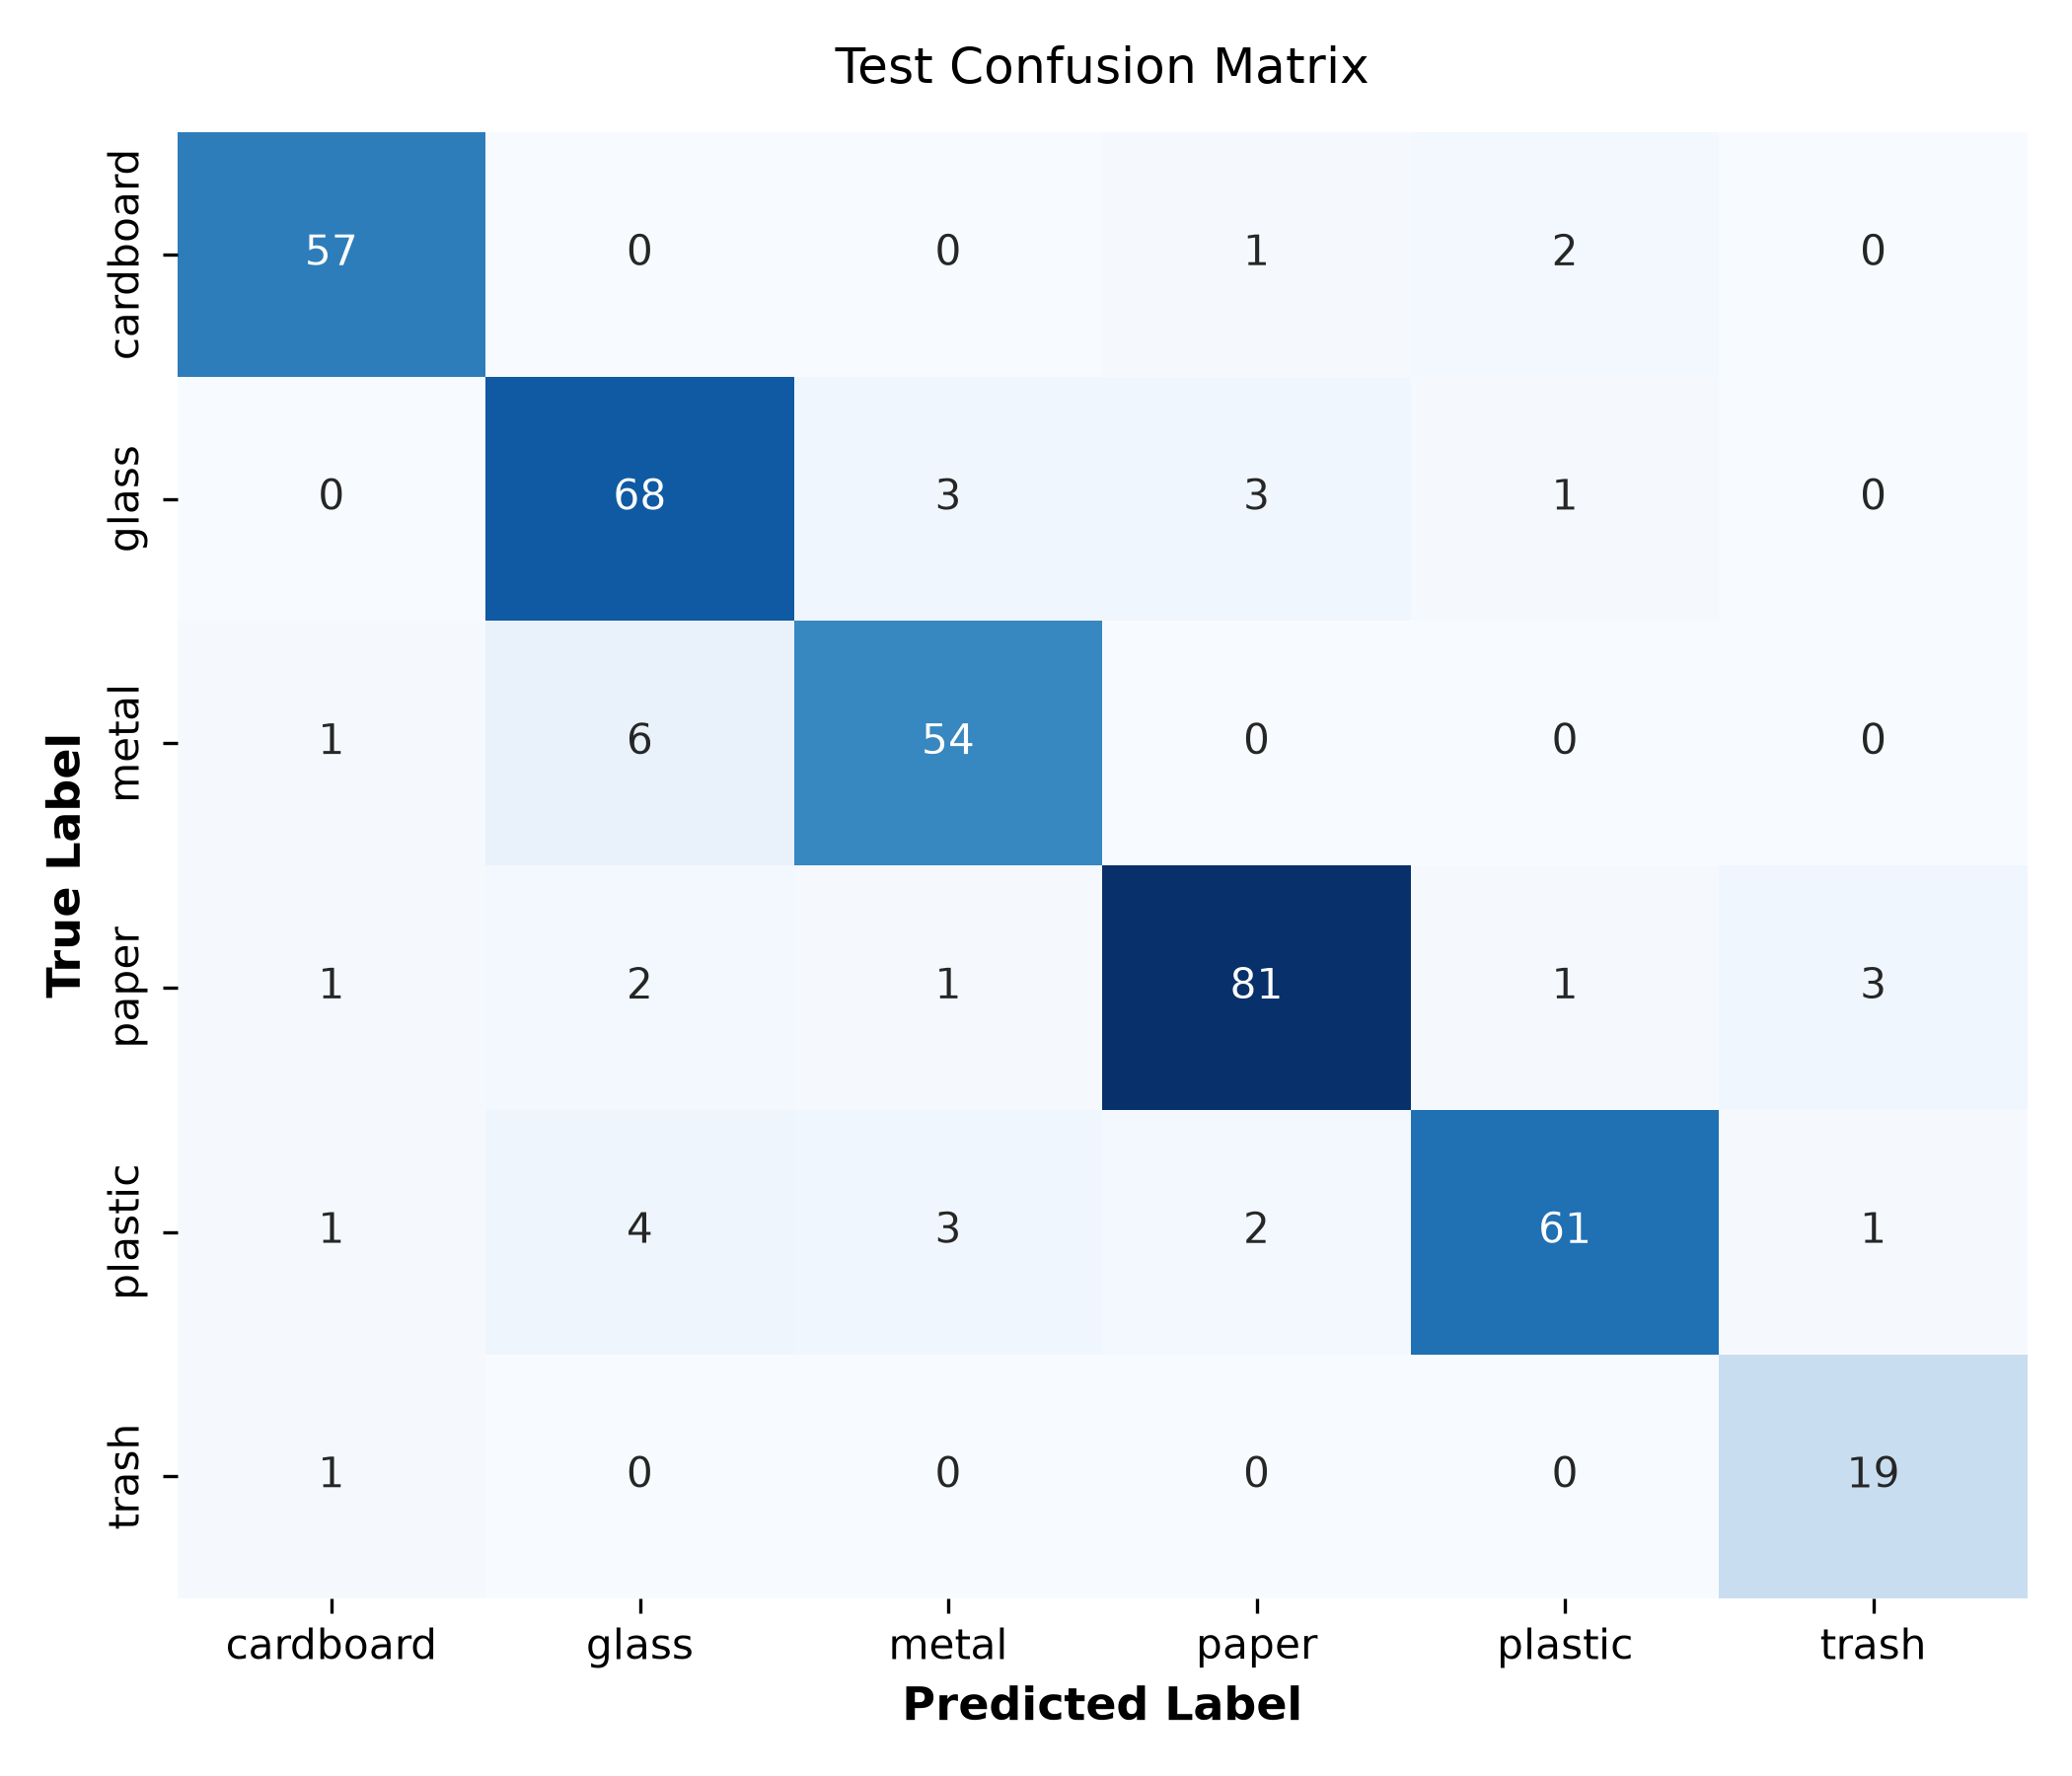
\includegraphics[width=\columnwidth]{figures/confusion-matrix.png}
\caption{Saved test confusion matrix. Rows are true classes and columns are predictions. No model inference was rerun for this report.}
\label{fig:cm}\end{figure}

\subsection{Probability Quality}
The saved multiclass log loss is 0.4599. The multiclass Brier score is 0.1828, using the mean over images of the sum of squared probability errors across all six classes. Expected calibration error (ECE) is 0.1325 with ten fixed confidence bins and sample-count weights. This is a noticeable confidence--accuracy gap, even though the model underwent calibration. The reliability diagram (Fig.~\ref{fig:rel}) shows underconfidence in several high-confidence bins. No paired uncalibrated test comparison was saved, so we do not claim a measured calibration improvement on this test set.

\begin{figure}[t]\centering
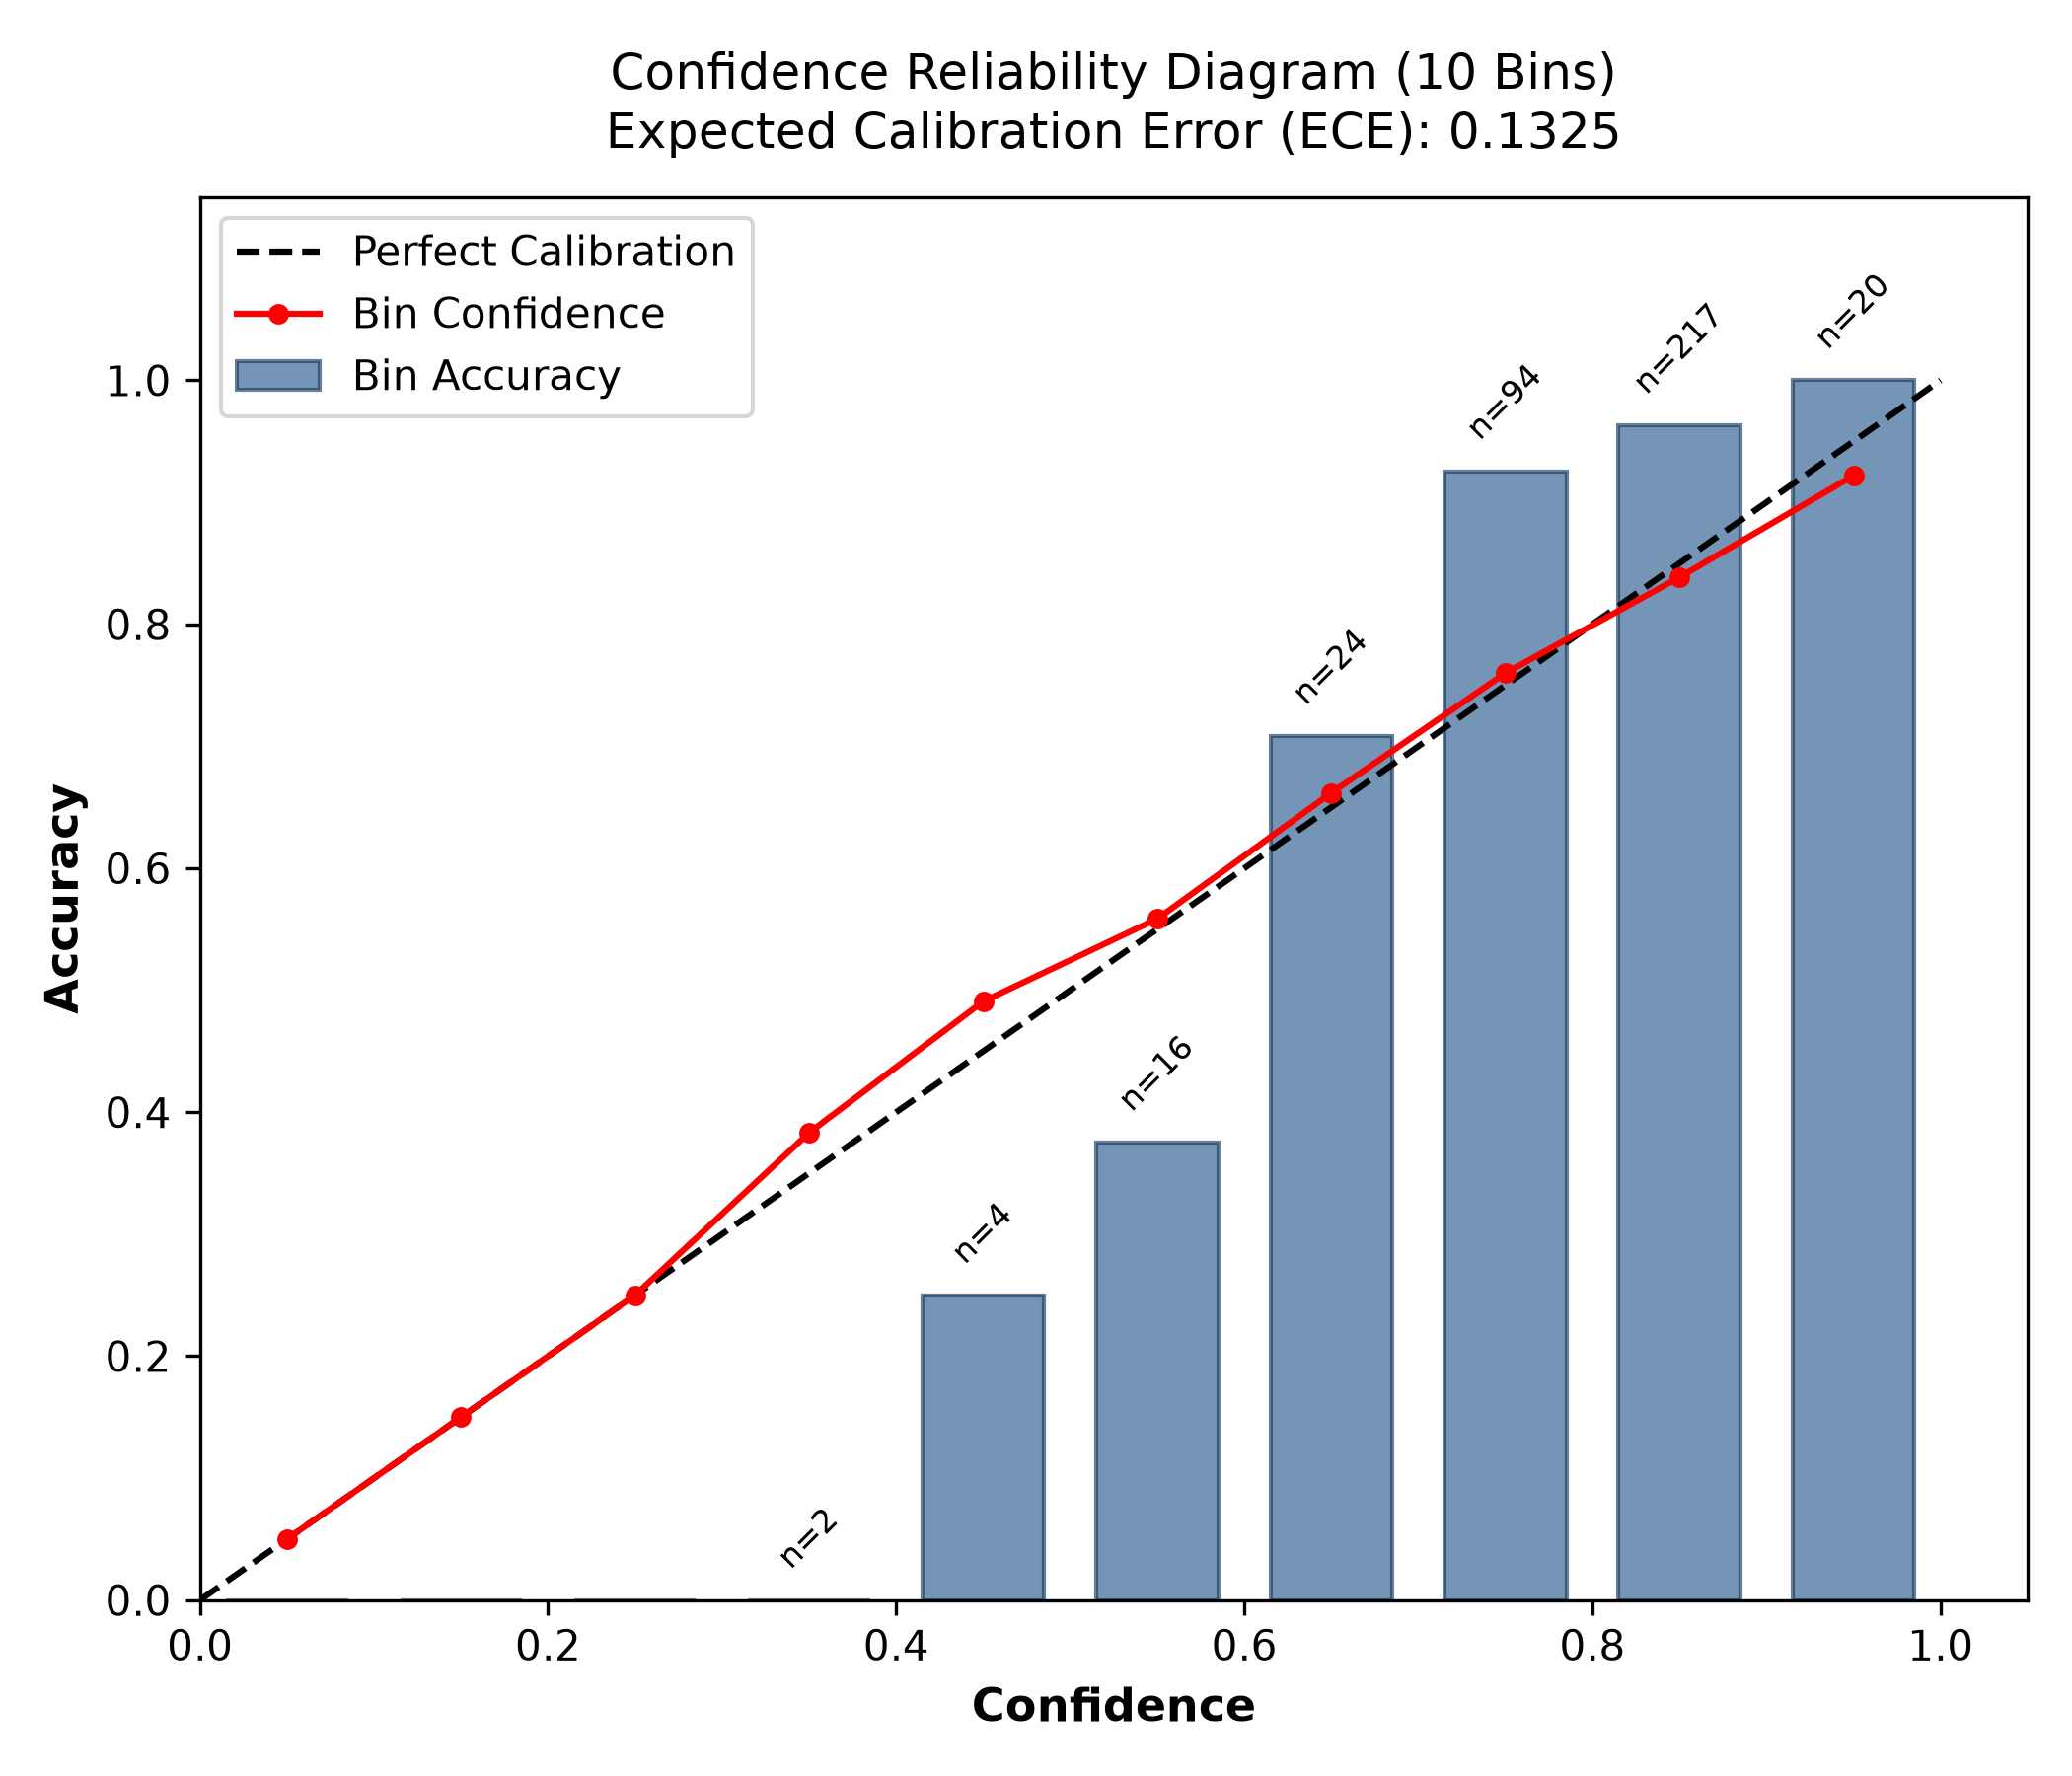
\includegraphics[width=\columnwidth]{figures/reliability-diagram.png}
\caption{Saved test reliability diagram. Calibration does not imply perfect probability reliability; ECE is 0.1325.}
\label{fig:rel}\end{figure}

\subsection{Coverage and Accepted Performance}
At the frozen threshold, six predictions abstain and 371 remain. Accepted accuracy is $339/371=91.37\%$, accepted macro F1 is 0.9129, and coverage is 98.41\%. The accuracy gain is 1.19 percentage points over unconditional accuracy, measured on a smaller accepted subset. It is not an improvement on all 377 predictions.

Five of the six abstained predictions are incorrect and one is correct. These include cardboard predicted as paper, glass predicted as metal, paper predicted as glass, and plastic predicted as metal or trash. The correct paper prediction is also withheld. Among all 37 errors, metal-to-glass confusion is the largest single off-diagonal count (six). Plastic accounts for 11 errors across other classes. These observations motivate future background and material-appearance analysis, not retuning on this test set.

\section{Demo, Reproducibility and Contributions}
The Gradio 6.30.0 application verifies and loads the original 66.3~MB artifact once, then delegates to the shared prediction function. It displays a class, six probabilities and a frozen-threshold uncertainty response. Clear resets the input and outputs; replacing an image clears stale results. Input bounds apply before feature extraction, but Gradio decodes uploads before the application callback. Gradio may retain temporary upload files after a browser session. Public sharing is disabled by default.

The integration follow-up removes a local substitute library and verifies the actual server. All 162 local tests pass with the original artifact present. CI exercises the real demo dependencies and skips the single artifact-specific test when the separately distributed binary is absent. Desktop and mobile inference checks use generated inputs and are functional tests, not a new accuracy benchmark.

Python 3.12 is the supported environment. The historical model-runtime lock pins Pillow 13.0.0. Gradio's constraint requires Pillow 12.3.0 in the demo lock; other base pins match. Six generated-image compatibility cases produced identical 2,760-dimensional features and predictions across those Pillow versions, which is bounded evidence rather than universal equivalence.

The preserved artifact SHA-256 is split below for readability:
\begin{center}\footnotesize\ttfamily
83b0658d5180c02d6f03dce835bb8e269\\
d6a89a493b6298a2bb00fd594f3b112
\end{center}
Experiment tables derive from committed JSON/CSV records. The repository is
\url{https://github.com/shourya2006/smart-waste-segregation}.

\begin{table}[t]\caption{Individual Technical Contributions}\centering
\begin{tabular}{lp{5cm}}\toprule
Member & Primary contribution\\\midrule
Om Yadav & Data verification and shared preprocessing\\
Aditya Bharadwaj & Baseline descriptors and cache validation\\
Shourya Bafna & Training protocol, SVM studies and integration fixes\\
Daksh Batra & Random Forest comparisons and refinement\\
Prajjwal Tripathi & Calibration, abstention and frozen evaluation\\
Saksham Mighlani & Demo, report and presentation assembly\\\bottomrule
\end{tabular}\end{table}

\section{Limitations and Phase 2}
First, TrashNet's controlled backgrounds and six known categories limit generalization. Multiple items, contamination, strong lighting changes and unfamiliar objects remain outside the demonstrated performance claim. Second, perceptual hashing can miss repeated objects at substantially different viewpoints. Third, class imbalance and small test supports limit certainty about minority-class behavior. Fourth, repeated exploration on the same training folds introduces selection bias, even though the outer test remains separate.

The original evaluation ran on an uncommitted working tree. Its historical source hash is preserved, but no snapshot of that exact tree exists in Git. The author's explanation attributes later differences to formatting and reporting changes; the exact historical source cannot be independently reconstructed. The fitted model, threshold and saved predictions remain unchanged.

Phase~2 should compare a frozen pretrained representation such as MobileNetV2 with these classical baselines, using an explicit augmentation and evaluation protocol. An independent everyday-photo set should probe lighting, backgrounds, unknown categories and mixed materials. The current test set is already observed and must not become a tuning set for further claims.

\section{Conclusion}
The selected handcrafted color and texture pipeline achieves 0.8999 test macro F1 and 90.19\% accuracy on the frozen TrashNet split. Validation-selected abstention reaches 91.37\% accuracy on 98.41\% of test images. Feature selection and representation design matter more than simply adding dimensions in these experiments. The result supports an educational photo classifier with visible uncertainty, while broader deployment and disposal guidance require additional evidence.

\balance
\bibliographystyle{IEEEtran}
\bibliography{references}
\end{document}
